\documentclass{article} %[draft]
\usepackage{calrsfs}
\usepackage{amssymb}
\usepackage{bm}
\usepackage{amsmath}
\usepackage{wrapfig} 
\usepackage{subfig}
\usepackage[acronym]{glossaries}
\DeclareMathAlphabet{\pazocal}{OMS}{zplm}{m}{n}
\DeclareMathAlphabet{\mathcal}{OMS}{cmsy}{m}{n}
\SetMathAlphabet{\mathcal}{bold}{OMS}{cmsy}{b}{n}
\newcommand{\bigO}{\mathcal{O}}
\usepackage{svg}
\usepackage{float}
\usepackage{adjustbox}
\usepackage{geometry}
\usepackage{pdfpages}
 \geometry{
 a4paper,
 left=25mm,
 right=25mm,
 top=30mm
 }

\makeglossaries

\newacronym{gpu}{GPU}{Graphics Processing Unit}
\newacronym{cpu}{CPU}{Central Processing Unit}
\newacronym{cuda}{CUDA}{Compute Unified Device Architecture}
\newacronym{fps}{FPS}{Frames Per Second}
\newacronym{lod}{LoD}{Level of Detail}
\newacronym{sfm}{SfM}{Structure from Motion}
\newacronym{mlp}{MLP}{Multi-Layer Perceptron}
\newacronym{nerf}{NeRF}{Neural Radiance Field}
\newacronym{dgs}{3DGS}{3D Gaussian Splatting}
\newacronym{bsp}{BSP}{Binary Space Partitioning}
\newacronym{sh}{SH}{Spherical Harmonics}
\newacronym{psnr}{PSNR}{Peak Signal-to-Noise Ratio}
\newacronym{ssim}{SSIM}{Structural Similarity Index Measure}
\newacronym{dbscan}{DBSCAN}{Density-Based Spatial Clustering of Applications with Noise}
\newacronym{ewa}{EWA}{Elliptical Weighted Average}

\usepackage{verbatim,shellesc}
\ShellEscape{cp /usr/local/share/latexmk/LatexMk ./LatexMk}


\begin{document}
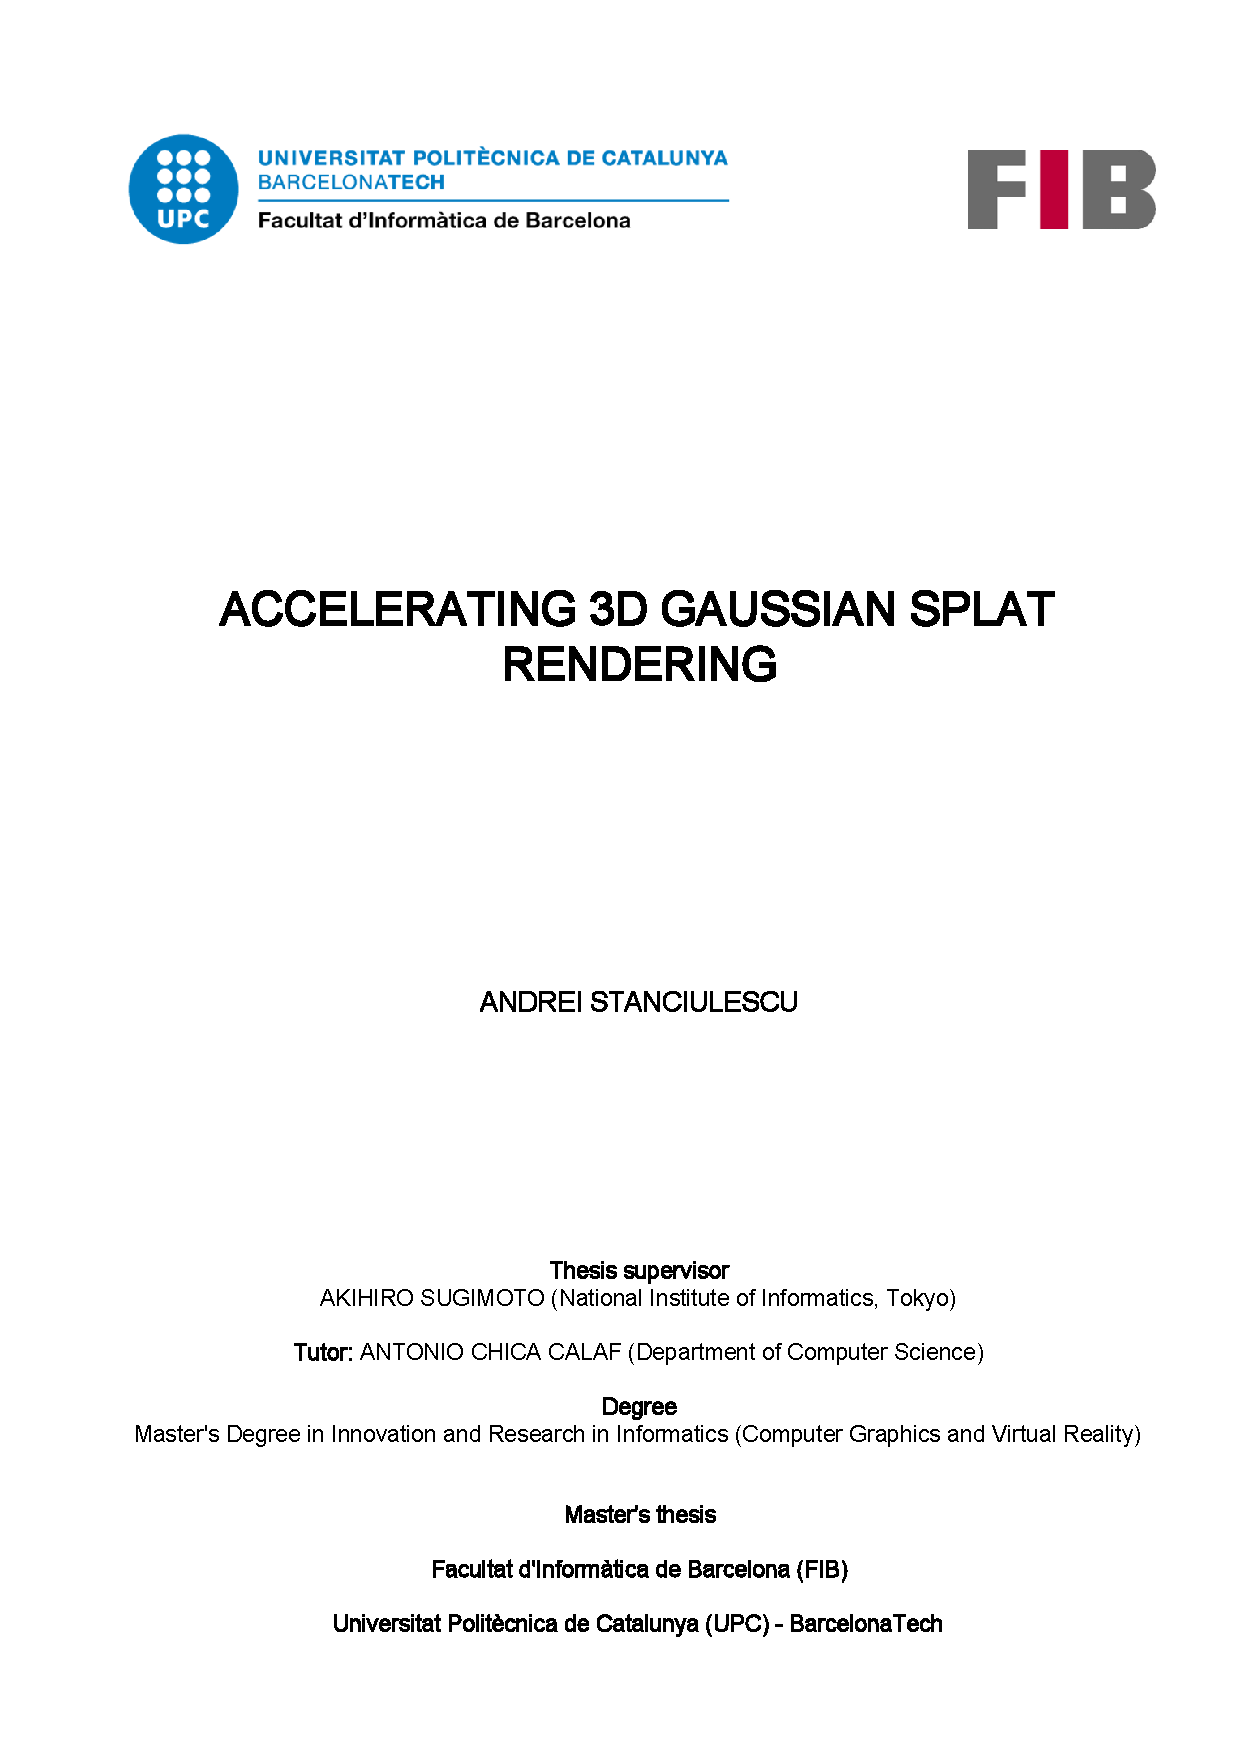
\includepdf[pages=1]{portada.pdf}

\begin{abstract}
    The 3D Gaussian Splatting method for 3D environment reconstruction from images brought significant advancements to photorealistic novel-view synthesis. It combines the advantages of primitive-based rendering with a differentiable renderer, thus obtaining state-of-the-art image quality and surpassing neural methods for scene representation in optimization and rendering speed. This is a significant step towards bringing these methods to real-time consumer applications, however, 3DGS still requires significant computing power which is not available in consumer devices. In this project, I will present a method for accelerating 3DGS rendering through a hierarchical Level of Detail structure that combines a regular octree subdivision with feature-based primitive clustering to obtain lower-detail representations. Also, I will present a level selection solution to maintain the desired detail granularity across the scene by computing a dynamic cut through the scene tree representation. This method achieves a reduction in the frame time between 14\% and 33\% by reducing the number of primitives in the scene to around 50\%, a reduction which maintains the image quality above 31 dB PSNR compared to the original reconstruction.
\end{abstract}
\newpage


\setcounter{tocdepth}{2}
\tableofcontents

\newpage
\glsaddall
\printglossary[type=\acronymtype, nonumberlist]

\newpage
\section{Introduction}
\newpage
\section{Related Works}

\subsection{Light Fields and Novel View Synthesis}
In the fields of computer graphics and computer vision, novel view synthesis refers to the problem of, given a relatively small set of model images from different camera positions
\newpage
\section{Overview}

In this project, I will present a new approach for accelerating Gaussian splatting rendering through a hierarchical Level-of-Detail structure. This is intended for consumer applications on consumer hardware, where the full scene cannot be rendered in real-time, and detail levels have not been provided with the optimized scene, so the simplifications have to be generated locally. All of the implementations presented in the previous chapter incorporate the levels of detail into the training algorithm, which allows them to optimize all of the levels, thus creating representations with very good quality. However, this requires a significant amount of resources that are not readily available on consumer hardware, so the availability of those LoDs depends on whether they were pretrained alongside the scene or not. Moreover, they also require the initial images for training the detail levels, which might not be readily available in consumer applications. 

The method I will present in the following chapters only requires the pretrained scene, from which it can generate an arbitrary number of levels without requiring additional training. Then, at render time, the detail levels for different parts of the scene can be selected based on the camera position and orientation, and the available hardware performance. The implementation takes advantage of the existing rasterization pipeline for 3DGS and introduces minimal changes to the render loop. Figure \ref{fig:system} shows a graphical representation of the pipeline I implemented in this project, highlighting in different colors the pipeline elements existing in the reference 3DGS implementation, and the additional pipeline steps introduced by my implementation.

\begin{figure}[H]
    \centering
    \includesvg[width=0.7\linewidth]{figures/system.svg}
    \caption{Overview of the implemented system.}
    \label{fig:system}
\end{figure}

\paragraph{}
The acceleration structure I propose in this project is built on a hybrid hierarchical space partitioning scheme based on insights from previous works on the topic. The root node of the scene represents the entire scene, which is incrementally subdivided into an octree up to a specified depth. This allows for an even distribution of nodes in the scene, and the maximum octree depth defines the lowest detail level of the simplification. Then, each octree leaf becomes the root node of a binary partitioning tree which will hold the merged and simplified Gaussians. Details on the partitioning structure will be presented in chapter 6.

I will also propose a new partitioning strategy for the Gaussians in the deeper nodes of the tree based on feature clustering, which, for this use case, performs better than previously proposed solutions that are solely based on Gaussian position. Also, because this method does not involve any training or fine-tuning, I will also propose a method for merging the Gaussians to create simplified representations and a comparison to the other methods in the literature. Details on this aspect will be discussed in chapter 5 of this document.

Then, I will discuss the method I used for combining the merging and partitioning algorithm to obtain a hierarchical level of detail structure, and how the appropriate levels are selected at runtime.

\paragraph{}
In Chapter 8 I will perform an analysis of the performance considerations taken into account when implementing this structure, how it fits into the existing 3DGS rasterization pipeline, and profiling the algorithm. Also, I will investigate its potential for further acceleration through earlier frustum culling. 

\paragraph{}
Lastly, I will present the experimental results in terms of image quality, rasterization speed, and required resources compared to the reference 3DGS implementation. Note that for this project, all of the experiments have been done on consumer hardware, as this is the intended use of this method, and not on workstation-grade GPUs like the other previously presented works. 
\newpage
\section{Rendering}
In this chapter, I will present the details of the rasterization pipeline for 3DGS, as introduced in the reference implementation. Because the Gaussians are rendered directly without any intermediate representation through other standard primitives, the process cannot take advantage of the existing geometry pipelines implemented on GPUs. In turn, it is based upon a tiling software rasterizer implemented as a CUDA kernel.

The render loop is made up of two main routines: the preprocessing stage and the rasterization routine, with a few intermediary steps in between for splat duplication, sorting, and assignment to tiles. This process takes as input the camera transformation and the Gaussian data and outputs the correct pixel color to a pixel buffer that allows the interoperability between CUDA and OpenGL. The only render call made to OpenGL is for a textured quad that fills the whole frame and is textured with the rasterized image. 

\subsection{Preprocessing}

As discussed previously, Gaussian primitives in 3DGS are defined by the following properties: mean $\bm{\mu} \in \mathbb{R}^3$, scale $\bm{S} \in \mathbb{R}^{3}$, rotation quaternion $\bm{q} \in \mathbb{R}^4$, opacity $\alpha \in \mathbb{R}$, and a set of spherical harmonics coefficients represented as an array of 48 floating point values, out of which 3 represent the base color, and the rest the specular details. Using this formulation, the distribution of a 3D Gaussian at any point in space $\bm{x}$ is the following \cite{ewa_splatting}:\[G(\bm{x} - \bm{\mu}) = e^{-\frac{1}{2}(\bm{x} - \bm{\mu})^T \Sigma^{-1} (\bm{x} - \bm{\mu})}\] This value is multiplied by the specific opacity of each Gaussian before being used for the last alpha-blending step. 

\subsubsection{Gaussian Covariance}
We can build the covariance matrix from the scaling matrix $S = diag(\bm{s}) \in \mathbb{R}^{3 \times 3}$ and the rotation matrix derived from the quaternion $\bm{q} = (x, y, z, w)$ as \cite{ye2023mathematicalsupplementtextttgsplatlibrary}:
\[
\bm{R} = \begin{bmatrix}
1 - 2 \cdot (y^2 + z^2) & 2 \cdot (xy - wz) & 2 \cdot (xz + wy)\\
2 \cdot (xy + wz) & 1 - 2 \cdot (x^2 - z^2) & 2 \cdot (yz - wx)\\
2 \cdot (xz - wy) & 2 \cdot (yz + wx) & 1 - 2 \cdot (x^2 + y^2)
\end{bmatrix}
\]

Then, we can build the 3D covariance matrix as $\Sigma = R S S^T R^T$. As the matrix is symmetrical, only the upper triangular region is stored. Now, the 3D covariance has to be projected to screen-space into a 2D covariance. A perspective transformation does not map a 3D Gaussian into a 2D Gaussian on the screen. For simplicity, the EWA splatting algorithm \cite{ewa_splatting} is used to approximate the perspective transformation by an affine local transformation using the first-order Taylor expansion at point $\bm{t}$, where $\bm{t}$ is the projected mean point of a Gaussian through the camera extrinsic matrix. Let $(f_x, f_y)$ be the focal lengths of the camera. Then we can obtain the Jacobian matrix of the perspective projection mapping at $\bm{t}$:
\[
\bm{J} = \begin{bmatrix}
f_x/t_z & 0 & f_x \cdot t_x / t_z^2\\
0 & f_y/t_z & f_y \cdot t_y / t_z^2
\end{bmatrix} \in \mathbb{R}^{2 \times 3}
\]
If the camera extrinsic matrix is:
\[
T_{cam} = \begin{bmatrix}
R_{cam} & t_{cam}\\
0 & 1
\end{bmatrix} \in \mathbb{R}^{4 \times 4}
\]
then we can finally compute the 2D covariance matrix of the projected Gaussian as:
\[
\Sigma_{2D} = \bm{J} R_{cam} \Sigma R_{cam}^T \bm{J}^T \in \mathbb{R}^{2 \times 2}
\]

At this point in the pipeline, the low-pass filter is applied to the covariance by ensuring that splats are at least one pixel in each direction using the following formula:
\[
\Sigma_{screen} = \Sigma_{2D} + \begin{bmatrix}
0.3 & 0\\
0 & 0.3
\end{bmatrix}
\]

The value of 0.3 is chosen somewhat arbitrarily, the reasoning being that when evaluating the ellipse of 99\% confidence interval of a Gaussian, which is at three standard deviations from the mean, the value of 0.3 would roughly translate to a 1-pixel dilation in both directions of the variance of the Gaussian. Other methods, such as the Mip-Splatting presented earlier, use values that are influenced by the Gaussian's dimensions and the frequency band limitations of the resolution the scene is rendered at.

\subsubsection{Splat geometric properties}

The inverse of the 2D covariance matrix $\Sigma_{2D}$ is a conic matrix that will be used later in the render routine to compute a Gaussian's influence at multiple locations on the screen.

From the eigenvalues of the 2D covariance $\lambda_1, \lambda_2$ where $\lambda_1 > \lambda_2$, we can then determine the minimum radius of a circle centered at the Gaussian mean that contains the 99\% confidence of the interval as $r = 3\sqrt{\lambda_1}$. Knowing the radius and the projected location of the Gaussian's center, we can then compute a screen-space bounding rectangle for the splat. 

From this bounding rectangle and knowing the dimensions in pixels of each tile in the rasterizer, we get the number of overlapped tiles, determining how many times the splat will have to be duplicated in the next step. This value, alongside the conic matrix, radius, projected center, and splat depth (the value of the Z coordinate in the viewport position) will be stored in global memory and passed to the next step.

\subsubsection{Splat color}
In order to represent variations in color based on different viewing directions on a single splat, the 3DGS implementation uses spherical harmonics. These are a set of functions defined on the surface of a sphere, which form an orthonormal basis, so any function defined on the surface of a sphere can be decomposed into a series of spherical harmonics of multiple degrees \cite{maths_for_physiscs}. For performance and storage considerations, this implementation uses harmonics up to degree $l=3$, as additional levels require more storage and only improve high-frequency details. For each splat, the viewing direction vector is normalized, then its components are used as input to the spherical harmonics function. The standard formulation for the spherical harmonics with the Condon–Shortley phase is used, and the coefficients are precomputed and stored in a table. When compositing the color for each channel, each term of the harmonic expansion is also multiplied by a learned coefficient which is produced by the scene optimization procedure. This allows control of various detail frequencies across the four harmonics degrees and the three color channels. 

\subsection{Splat duplication and sorting}
In order for the tiling rasterizer to execute efficiently, each tile workgroup needs to have all the necessary data in a contiguous location in memory. Since splats can overlap multiple tiles, this introduces the need to duplicate splat data for each tile and arrange it appropriately in the device memory. To execute some of these operations, the implementation uses the CUB library, which provides state-of-the-art parallel primitives for the CUDA programming model. 

The first step is to determine the total number of splats after duplication, and the array offsets for duplicating in memory. This is done using the overlapped tile values computed in the previous step, on which is applied an inclusive prefix sum scan. This computes, for each element, the sum of all previous values in the array, including itself, and stores the sum in a new results array. This means that given an array of integers of size n $\bm{x} \in \mathbb{N}^n$, the resulting inclusive prefix sum array $\bm{s}$ is:
\[
\bm{s}_k = \sum_{i=0}^{k} \bm{x}_i
\]
The values in this array will then provide the necessary offsets for duplicating the splat data in memory, and the amount of memory that has to be allocated. The formulation above, implemented on the CPU, has a time complexity of $\bigO (n)$. However, taking advantage of the fact that the data is stored on the GPU, the implementation uses the parallel version of this prefix scan routine \cite{Merrill2016SinglepassPP}, which takes advantage of the massively parallel capabilities of GPUs and can perform this sum in $\bigO (\log_2 n)$ steps by aggregating partial sums.

The next step is duplicating the splat IDs and preparing them for sorting. The tiling rasterizer needs the splats to be ordered by depth, and the data in global memory needs to be contiguous for each tile. To achieve this, the duplicated IDs will be sorted by a set of precomputed keys. During duplication, keys containing the overlapped tile ID and the splat depth are generated for each duplicated splat ID. This means that each duplicated splat will be associated with a unique tile. We wish the arrangement in memory to be done first by splat ID, so splats overlapping the same chunk are contiguous in memory, and then by depth inside each block, so the rasterizer does not have to perform any further sorting. Thus, the keys are built as 64-bit values, where the higher 32 bits represent the overlapped splat ID, and the lower 32 bits represent the splat depth, as shown in figure \ref{fig:sortkey}. Because the tile ID occupies the higher-significance bits, it will have priority during sorting.

\begin{figure}[H]
    \centering
    \includesvg[width=0.95\linewidth]{figures/sorting key.svg}
    \caption{Sorting key structure for splat ordering.}
    \label{fig:sortkey}
\end{figure}


After sorting, the keys will have a structure as seen in figure \ref{fig:sortedkey}, where the first half of each cell is color-coded by tile ID, and the gradient of the second half shows the depth. To sort the values in device memory by keys, the most efficient method is to use RadixSort \cite{radix_sort}, also implemented in the CUB library. It performs a least significant digit sorting, so the values are sorted in multiple passes, from the least significant digit to the most significant digit. Even though the depth component of the key is a floating point number, it will be interpreted as an integer, which is not an issue since the depth always has the same sign, so ordering as an integer representation produces the same result. The number of passes necessary for sorting depends on the number of digits of the key with the highest value, and it scales linearly with the number of sorted elements and performs very efficiently on the GPU architecture. Because usually, the value for the tile ID does not take up the whole 32 bits allocated for it in the sorting keys, we can determine the highest non-zero bit across all keys and terminate the sorting there, which might reduce the number of necessary sorting passes, depending on the stored values. In my testing, this extra check eliminates one of the passes, resulting in a small performance improvement.

The last step before calling the rasterization routine is to determine, for each tile, the start and end range of its data in the global splat ID array. Ranges are also shown in figure \ref{fig:sortedkey}.
\begin{figure}[H]
    \centering
    \includesvg[width=0.95\linewidth]{figures/sorted_keys.svg}
    \caption{Sorted keys showcasing tile ranges.}
    \label{fig:sortedkey}
\end{figure}

\subsection{Splat Rasterization}
The rasterizer used in the reference 3DGS implementation cannot take advantage of the hardware graphics pipeline for processing splat primitives, so a tiled software rasterizer is used instead. This means that the rasterization is done through a programmable CUDA kernel. The screen is split into a grid of $16 \times 16$ pixels each, and the image on each grid block, or tile, is generated independently of the other tiles and composed in the end in the output buffer, thus the need for splat duplication done in the previous step. The render kernel is launched as a grid of blocks, and each block processes one screen tile and is made up of $16 \times 16$ threads. This means that there is one thread processing each pixel on the final render. 

Inside every block, all threads will process all the splats assigned to the tile. Global memory accesses are costly and can significantly stall the kernel's execution and would be very wasteful especially if all threads need to access the same data. To avoid this memory access overhead we can take advantage of the local shared memory of each Streaming Multiprocessor \cite{cuda_ref}, which is however much smaller than global memory and cannot fit all splat data at once. To go around this limitation, the image can be composed in multiple passes, each pass processing 256 splats assigned to the tile. At the start of a pass, each thread loads into local shared memory (L1 cache) the screen position, conic matrix, and splat ID. Then, a synchronization barrier is used to ensure all data is loaded before proceeding to the next step. After synchronization, each thread in the block processes all the splats collected in local memory and computes their influence on their assigned pixel in the render. After the color blending is done, the block loads and processes the next batch of 256 splats and the process repeats until all splats assigned to the tile have been rasterized.

The influence of a Gaussian on a specific pixel is determined by the distance between the 2D Gaussian on the screen and the pixel location, which is passed through an exponential falloff function. Because the EWA volume splatting algorithm projects 3D Gaussians to screen as ellipses, we can define the following radial basis function:

\[
r(\bm{d}) = \bm{d}^T \bm{Q} \bm{d}
\]

where $\bm{d} \in \mathbb{R}^{2}$ is the component-wise distance vector between the center of a splat and the pixel position and $\bm{Q} \in \mathbb{R}^{2 \times 2}$ is the conic matrix of the splat (i.e. the inverse of the 2D covariance matrix). Then, opacity of a splat centered at point $\bm{s} = (s_x, s_y)$ evaluated at a pixel with center $\bm{p} = (p_x, p_y)$ is:
\[
\alpha_{\bm{p}} = \alpha \cdot e^{-\frac{1}{2}r(\bm{s} - \bm{p})} 
\]

where $\alpha$ is the learned base opacity of the Gaussian (i.e. the opacity at the center of the splat). 
% Figure shows a graphical explanation of the splat sampling procedure. 
% \begin{figure}[H]
%     \centering
%     \includesvg[width=0.6\linewidth]{figures/splat_sampling2.svg}
%     \caption{Splat opacity sampling.}
%     \label{fig:sampling}
% \end{figure}

Splats are processed front to back, and the contribution of each splat is accumulated for each pixel following an alpha-blending compositing formula. In the end, the color of a pixel $k$ is given by the following formula:
\[
\bm{C}_k = \sum_{n < N} \bm{c}_n \cdot \alpha_n \cdot T_n \text{ where } T_n = \prod_{i < n} (1 - \alpha_i)
\]

Here, $N$ designates the number of splats overlapped by the tile that the thread processing pixel $k$ is assigned to, and $\bm{c}_n$ is the color of splat $n$. To ensure better performance splats with computed opacity lower than $\frac{1}{255}$ are skipped, and the color compositing can be terminated early if the remaining transmittance coefficient $T_n$ is lower than $10^{-4}$, as the pixel is considered to have reached "full" opacity and any further contributions are insignificant.

\subsection{Performance profiling}
The scope of this project is to propose an acceleration structure for 3DGS rendering, so after explaining the rendering pipeline, it makes sense to also perform a short performance analysis in order to identify potential bottlenecks and the routines that would most benefit from potential speedups. The profiling has been performed on the "Train" scene of the \textit{Tanks and Temples} dataset \cite{Knapitsch2017}, using one of the standard training camera positions. Data has been collected using NVIDIA Nsight Compute, which offers launch statistics, timing, and bottleneck statistics on profiled CUDA kernel launches, and will be an indispensable tool for this project. All the experiments for this project have been performed on a laptop with an NVIDIA RTX 3050 Ti GPU with 4GB of VRAM running at 35W.

Figure \ref{fig:init_profile} shows the render pipeline profile. The final render routine takes up around 65\% of the execution time of the pipeline, indicating that it would be the best candidate for optimization, followed by the sorting at 13.7\% and 6.17\% for the duplication and key generation. However, Nsight Compute reports a compute throughput of over 90\% for the render routine, so optimizing the code will most likely result in minimal improvements, and the RadixSort routine is highly optimized already for the CUDA architecture. This indicates that if we wish to maintain the same pipeline for rendering, the most obvious way to increase the performance is to render fewer Gaussians in each frame. 

\begin{figure}[H]
\makebox[\textwidth][c]{
    \centering
    \begin{minipage}{0.5\textwidth}
        \centering
        \includesvg[width=\linewidth]{figures/init_profile.svg}
        \caption{Render pipeline routine duration.}
        \label{fig:init_profile}
    \end{minipage}\hfill
    \begin{minipage}{0.5\textwidth}
        \centering
        \includesvg[width=\linewidth]{figures/speedup.svg}
        \caption{Render routine speedup when reducing the number of rendered Gaussians.}
        \label{fig:speedup}
    \end{minipage}
    }
\end{figure}

To investigate the potential improvements of reducing the number of rendered Gaussians, I profiled the render routine on the same scene, rendering all the Gaussians, half of the Gaussians, and lastly a quarter of the Gaussians. Figure \ref{fig:speedup} shows the speedup obtained by reducing the number of Gaussians in the scene, indicating an almost linear relation between render time and the number of primitives. Of course, the relationship is not always linear and further decreasing the number of primitives produces diminishing returns, as kernel launch overheads become more relevant. However, just arbitrarily removing Gaussians from the scene is obviously not a good solution, so there is a need to create a scene simplification structure, which I will present in the following chapters.

\newpage
\section{Gaussian Merging}
As discussed in the previous chapter, one way to accelerate 3DGS rendering is by reducing the number of primitives in the scene, which can be done using simplified representations, similar to levels of detail on triangle meshes. Some implementations presented in the literature review propose very simple methods for Gaussian merging, such as averaging all properties. This technique is not accurate for all properties, but in those cases, it is a good starting point, as the simplified representations are also trained during the scene optimization process. However, for this implementation, I need to find an approach that produces quality results without further fine-tuning, because the simplifications are used directly as they are generated at runtime. In this chapter, I will present the approach used in this implementation for merging two Gaussians into one primitive in order to obtain scene representations with fewer Gaussians.

\subsection{Spherical Harmonics}
The main use of the merged Gaussians is to replace primitives far away from the camera with a simplified representation in order to increase performance by decreasing detail in areas where the loss in quality is not that noticeable. Thus, the intended use of the simplification is distant areas from the camera. In this situation, the original Gaussians will only take up a reduced area on the screen, which would be equivalent to rendering them at a lower resolution if they were closer to the camera. Using the insight from studies on antialiasing for Gaussian splatting, a good option for band-limiting the rendered primitives is to apply a box blur filter that acts as a low-pass filter. Applying a 2D box blur filter to a patch of pixels on the screen is done by convolution of the initial image with a $3 \times 3$ kernel with the following formulation when applied in image space \cite{box_filter}: 
\[H = \frac{1}{9} \begin{bmatrix}
1 & 1 & 1\\
1 & 1 & 1\\
1 & 1 & 1
\end{bmatrix}\]

As expected, the blur used to subsample the projected primitives to improve aliasing takes the average of neighboring pixels. That indicates that in order to get a similar representation from a single primitive, a good choice for the color is the mean of the initial primitives. However, taking a simple average of the color would ignore the different contributions different Gaussians have to the final image on the screen. Some implementations propose determining the visual importance of a Gaussian as the amount of overlapped pixels over all training images. While this is a relevant metric, the method I am proposing is intended for generic use on 3DGS scenes, not necessarily aiming for the highest metrics on a set of predetermined camera positions. For this reason, I chose to consider the relative contribution of a Gaussian as a function of its learned opacity and volume. Thus, I chose the following formulation to define the weight of a Gaussian $i$: $w_i = \alpha_i \cdot V_i$, where $V_i = s_x\cdot s_y \cdot s_z$. Because the actual color is computed in every frame depending on the camera position, I will blend the Gaussians using a weighted mean on the arrays of SH coefficients. The coefficients are separated by color, so the weighted mean can be applied to each channel individually and will provide the desired result when recomposing the color from the new SH coefficients and viewing direction. 

\subsection{Opacity}

In order to compute the opacity of the merged Gaussian, I am using an approach similar to the one in \cite{kerbl_hierarchy}. One thing to note is that the opacity property of Gaussians defines the maximum opacity at the center of the splat and is the value from which the splat's opacity falls following a Gaussian curve towards the edges of the splat. However, when two Gaussians projected to the screen overlap, the perceived opacity across them does not follow a Gaussian distribution, as the two opacities are composed over the overlapping region, so the falloff is slower than a Gaussian. 

It is important to model this behavior, otherwise the merged primitive will have lower perceived opacity, and applying the merging procedure hierarchically would result in significant opacity loss across the scene. Consider two partially overlapping Gaussians projected on the screen as in figure \ref{fig:blendfig}. A scanline plotting the opacities across the space occupied by the two splats will produce the profiles shown below, where figure \ref{fig:opacity_sum} shows the sum of opacities generated by the distributions, and figure \ref{fig:perceived_opacity} shows the total opacity saturated at 1, as that is the maximum opacity accepted by the rasterization routine. Note the plateau around the center of the two splats generated by the sum of the two decaying opacities, which cannot be directly modeled by a Gaussian distribution. 

\begin{figure}[H]
    \centering
    \includesvg[width=0.5\linewidth]{figures/blending.svg}
    \caption{Scanlines across the initial Gaussians and the merged one.}
    \label{fig:blendfig}
\end{figure}

However, the shape of the function above the $\alpha = 1$ line is not important, as the opacity will be saturated at 1. This means that this behavior can be modeled by a single Gaussian distribution with a peak higher than 1, as shown in figure \ref{fig:merged_model}. This is an oversimplification of the potential situations for Gaussian opacity merging, and the height of the distribution would depend on many variables such as the distance between primitives and their scales. However, it showcases the need for primitives after merging to have an opacity greater than 1 to simulate a slower fall-off.

\begin{figure}[H]
\makebox[\textwidth][c]{
    \centering
    \begin{minipage}{0.4\textwidth}
        \centering
        \includesvg[width=\linewidth]{figures/opacity_sum.svg}
        \caption{Scanline opacities.}
        \label{fig:opacity_sum}
    \end{minipage}\hfill
    \begin{minipage}{0.4\textwidth}
        \centering
        \includesvg[width=\linewidth]{figures/perceived_opacity.svg}
        \caption{Perceived opacity.}
        \label{fig:perceived_opacity}
    \end{minipage}\hfill
    \begin{minipage}{0.4\textwidth}
        \centering
        \includesvg[width=\linewidth]{figures/merged_model.svg}
        \caption{Merged opacity model.}
        \label{fig:merged_model}
    \end{minipage}
    }
\end{figure}

I chose to use a similar approach to the \textit{Hierarchical 3D Gaussian Representation} paper from INRIA, but changing the splat surface to Gaussian volume, as it would be a more reliable metric for any arbitrary view in the scene. Thus, the opacity of a merged Gaussian is the following:
\[
\alpha_m = \frac{\sum_i^N w_i}{V_m}
\]
where $V_m$ is the volume of the new Gaussian from its covariance matrix, as will be explained in the next subchapter, the weights $w_i$ are the same as for the color merging.

\subsection{Mean and Covariance}
The most difficult properties to merge for Gaussian primitives are the geometric ones, such as mean and covariance. Especially the covariance, it defines both the spread of the distribution and its directions, i.e. the orientation of the Gaussian in space. A lot of research has gone into reducing the dimensionality of Gaussian Mixture Models, both from a purely analytical perspective \cite{gaussmerge2} and for use in hierarchical photon mapping \cite{gaussmerge1}. Considering any arbitrary normalized weights $w_i'$ assigned to a set of N Gaussians, the mean and covariance of the merged Gaussian are the following:
\[
\overline{\mu} = \sum_{i \leq N} w_i' \mu_i
\]
\[
\overline{\Sigma} = \sum_{i \leq N} w_i'(\Sigma_i + (\mu_i - \overline{\mu}) (\mu_i - \overline{\mu})^T) 
\]

This method aims to minimize the Kullback–Leibler divergence, which measures how much two probability distributions differ. The formulas above are also used by \cite{kerbl_hierarchy} to generate their intermediary nodes, but note that the scene training algorithm then optimizes the generated nodes. During testing, I implemented this merging approach but found that a direct implementation of the formulas above results in Gaussians that have lower volume than expected, so applying the same approach on multiple levels resulted in significant gaps appearing in the scene. Note that at the time of writing, the implementation of \cite{kerbl_hierarchy} was not published, so there was no reference to any pre- or post-processing they are doing to achieve the results described. Also, their very good quality metrics are very likely to be due to the extended training process after the merged Gaussians are generated.

In order to test an alternative to the method above, I chose to implement a covariance merging approach based on the volumetric coverage of the combined Gaussians. The challenge when merging primitives is to get a similar shape to the initial distributions and fill in the same space occupied by them. To achieve this, I chose to follow an approach that analyzes the volumetric extent of the composed Gaussians and tries to reproduce the same volumetric coverage using only one distribution. 

Given a set of $N$ 3D Gaussian distributions, the first step is to determine their volumetric coverage, which is the space they occupy inside their 99\% confidence interval. I chose to use this interval as it is the same one that is used after the primitives are projected to determine their on-screen bounds. From the eigenvectors of the covariance matrix, we can determine the axes of the confidence ellipsoid, and by scaling these vectors by a factor of 3, we get the extent needed to cover the desired confidence interval. Given the scaled vectors $\bm{s_1}, \bm{s_2}, \bm{s_3}$ that represent the ellipsoid axes and the center point of the Gaussian $\bm{\mu}$, I can generate a coverage point cloud $P$ defined as 
\[P = \{\bm{\mu}, \bm{\mu} + \bm{s_1}, \bm{\mu} + \bm{s_2}, \bm{\mu} + \bm{s_3}, \bm{\mu} - \bm{s_1},\bm{ \mu} - \bm{s_2}, \bm{\mu} - \bm{s_3}\}\]
which contains the center point and the ellipsoid vertices. This procedure is applied to all the primitives that are going to be merged, then we concatenate the sets of points generated by them:
\[Q = \bigcup_{i=1}^N P_i\]
The final volumetric coverage point set will contain $7N$ points. To get the merged Gaussian mean, we will take the weighted average of these positions, the weights being the same as for the other properties before:
\[
\bm{\overline{\mu}} = \frac{1}{\sum_i^{7N} w_i} \sum_{\bm{p} \in Q} w_p\bm{p} 
\]

The weights for all 7 points generated by one Gaussian are the same. Then, to compute the equivalent Gaussian spread, we only need to compute the covariance of the point set. Let the matrix $D \in \mathbb{R}^{7N \times 3}$ be defined as:
\[
D_i = Q_i - \bm{\overline{\mu}}, 1 \leq i \leq 7N
\]
and the diagonal weight matrix $W = diag(\bm{w}) \in \mathbb{R}^{7N \times 7N}$. Then, the weighted covariance matrix \cite{weighted_mean} is defined as:
\[
\Sigma = \bm{DWD^T}
\]

With the two formulas above we have the necessary information to describe the new distribution. Figure \ref{fig:pca2d} shows a simplified 2D representation of the coverage points and the computed resulting distribution for four Gaussians placed in different configurations in space.

\begin{figure}[H]
    \centering
    \includegraphics[width=0.7\linewidth]{figures/pca2d.png}
    \caption{Examples of computed point spread.}
    \label{fig:pca2d}
\end{figure}

The gray lines show the confidence ellipse of the initial Gaussians, and the dots show the distribution centers and ellipse vertices. The green line represents the confidence ellipse of the merged Gaussian, and the blue and red lines represent the covariance matrix eigenvalues. We can see that for Gaussians that are close together, the distribution spread follows the general shape. However, when the primitives are spread apart, the resulting merged Gaussian covers a significant amount of empty space. This highlights the necessity of a good selection mechanism for choosing the candidate Gaussians for merging. Ideally, we would like the primitive to be compact and without empty spaces between them.
\newpage
\section{Spatial Partitioning}
Since in the previous chapter I presented the method for merging 3D Gaussians and outlined some potential issues, the focus of this chapter is to discuss scene partitioning methods, which in the end will be the criterion for selecting groups of primitives for merging. I will first go over two well-known methods in computer graphics that have been explored by other publications on this topic, then present a novel approach and justify its advantages for this application in particular. 

\subsection{Octrees}
Octrees are one of the simplest forms of space partitioning in computer graphics. Usually, the root node of the tree represents the entire axis-aligned bounding box of the model or scene to be partitioned. Then, the node is split into $2 \times 2 \times 2$ nodes, each axis of the box being split simultaneously at its midpoint, resulting in 8 children nodes of equal sizes. The procedure then repeats recursively for all newly generated nodes until a stopping criterion is met. The criterion for stopping the subdivision could be reaching a maximum depth in the tree, reaching a minimum dimension of the leaf nodes, or it could depend on the number of primitives in the leaves since at some point subdividing further would not be beneficial for the application. Every time a node is subdivided, the primitives contained by the parent will be distributed between the children based on the bounding box intersection. Usually, primitives are stored only in the leaf nodes, and the set of primitives contained by an intermediary node can be determined by traversing its subtree. 

The octree can be used either as a structure for partitioning point data, such as vertices in a triangle mesh or a point cloud, or they could be the implicit representation of the data, for cases in which the information is better displayed as voxels than point geometry. Moreover, this kind of structure can be useful for queries in occlusion tests, collision detection or ray tracing.

Being a regular structure, octrees have some advantages. For example, the locations of the splitting planes are predetermined, and the size of the node can be determined during traversal from the size of the root node and the path taken through the tree \cite{RTR4}. However, their regularity comes at a cost if the scene or model does not have a somewhat uniform distribution of primitives inside its bounding box. Since nodes are always generated at half the dimensions of the parent and at predetermined positions, many generated nodes may be empty. Moreover, clusters of very close-by primitives may take a large amount of recursion steps to be split into different nodes, because the splitting planes are generated at specific positions and do not adapt to the data. Figure \ref{fig:octree_diff} shows two examples of octree subdivisions for a set of Gaussians (shown in 2D as a quadtree for easier representation), the illustration on the right highlights the inefficiencies of regular space division, as many nodes end up empty.

\begin{figure}[H]
    \centering
    \includesvg[width=0.9\linewidth]{figures/octree_diff.svg}
    \caption{Octree (quadtree for simplicity) examples for different cases of primitive organization in space. Empty nodes are shown in red.}
    \label{fig:octree_diff}
\end{figure}

To determine the repartition of Gaussians inside nodes, I am using only the center point of the Gaussian, and determining in which one of the eight children each primitive should be distributed. I experimented with considering the bounding box of the confidence ellipsoid and duplicating Gaussians where more nodes overlap, but this leads to an exponential increase of primitives in the acceleration structure. The method I have settled with is using the center point for node assignment and the AABB of the confidence ellipsoids to determine node bounding boxes used in rendering and generating the dynamic LoD. Differences between the node bounds and the computed bounding box for rendering can be seen in Figure \ref{fig:octree_bbox}.

\begin{figure}[H]
    \centering
    \includesvg[width=0.5\linewidth]{figures/octree_bbox.svg}
    \caption{Octree (quadtree for simplicity) showing node bounds and the node AABB computed from confidence ellipsoids.}
    \label{fig:octree_bbox}
\end{figure}

\subsection{BSP Trees}
Binary space partitioning trees are similar to octrees, the main difference being that each node is split into only two child nodes. Also, research on space partitioning for 3DGS suggests that a median split works well for this kind of scene. This approach implies splitting each node along the longest axis of its bounding box. As before, bounding boxes are axis-aligned, just like the splitting planes. To find the splitting plane, all the primitive centers are projected on the longest axis, sorted, and then the median position can be found, through which we will split the node, as shown in figure \ref{fig:bsptree_split}. Then, given that the projected positions are already computed, it is easy to distribute the primitives between the two children. Similarly to the octree, primitives are only stored in the leaf nodes. 

\begin{figure}[H]
    \centering
    \includesvg[width=0.9\linewidth]{figures/split.svg}
    \caption{Node subdivision for BSP tree showing projected centers on the longest axis and the split plane with a red dotted line.}
    \label{fig:bsptree_split}
\end{figure}

Because the positions of the splitting planes are not predetermined, the data structure needs additional storage to hold the information about its volume. On the other side, using a median splitting plane ensures that the final structure is a balanced tree, and there are no empty nodes. Even though BSP trees might need more depth than an octree to partition all primitives, this highly depends on the distribution of the primitives, as can be seen in figure \ref{fig:bsptree_diff}.

\begin{figure}[H]
    \centering
    \includesvg[width=0.9\linewidth]{figures/bsp.svg}
    \caption{BSP tree examples for different cases of primitive organization in space. No empty nodes compared to octree.}
    \label{fig:bsptree_diff}
\end{figure}

Other than the splitting method, for this implementation I am using the same approach as with the octrees, distributing primitives based on center position, and computing an additional bounding box based on the confidence ellipsoid. From my experiments, I have found that using a BSP strategy for generating the LODs gives more natural results since all leaf nodes differ in depth by one at most, so when generating a cut in the tree for creating the appropriate LOD, primitives tend to be more uniformly simplified, instead of having high-frequency Gaussians stuck in higher levels in the tree, which would require more simplification steps to be reached. Also, this structure allows for finer transitions between levels, since only two Gaussians are merged at a time, instead of eight.

\subsection{Hybrid Partitioning}
In this last section, I will present a hybrid space partitioning algorithm that I have implemented for this application, taking into account the advantages and disadvantages observed in the two approaches presented above. This method proved to produce better quality results, which will be discussed in a later chapter.

The first part of this approach involves the initial space subdivision, which is intended to result in a uniform distribution of nodes throughout the scene. Because these nodes are very coarse and contain a high count of primitives, they will not be used for generating the levels of detail. Instead, they are used as a starting point for the second subdivision step. This is why for this initial step I chose to use an octree partitioning approach, up to a specified depth, which is determined usually by the scene complexity.

For the second part of the partitioning, the primitives have to be more carefully grouped into nodes. When generating the LoDs, the distribution of Gaussians in nodes determines the order in which they will be merged, and because there are no further scene optimization steps applied after this, creating quality merged primitives is essential for reliable LoD representation. As discussed above, binary space partitioning is advantageous when considering that the stored Gaussians have to be merged, as we have more flexibility in determining the distribution of primitives in nodes. Moreover, binary splitting allows for finer transitions and more possible intermediate representations, as we have more interior nodes than an octree. 

When merging the primitives as explained in the previous chapter, the best results for merged Gaussians are obtained when the initial primitives have similar properties, whether it is spatial coherency or color similarity. This is because, for Gaussians clustered in space, the resulting distribution will approximate well the volumetric coverage, and for color similarity the resulting color will not deviate too much from the appearance of the initial Gaussians. While the median split method works well in evenly clustering spatial structures, in this implementation I will explore clustering-based methods for distributing Gaussians in the children nodes of the tree.

What I want to achieve in this step of space subdivision is a distribution in which, for a parent that is split into two children, the variance of the primitives inside nodes is low, while the variance between nodes is high. Because both position and color should be taken into consideration, each Gaussian is described by a feature vector $\bm{v} = (x, y, z, r, g, b)$, where the color is taken as the first spherical harmonic coefficient on each channel, as that is the one describing the base color of the primitive, and introducing multiple degrees of the harmonics in the clustering would both be inefficient in terms of computation complexity and would bias the clustering towards color and variations based on viewing position. Also, it is worth mentioning that the position is relative to the node center and normalized to the extent of the node's bounding box, so the clustering would not be biased towards position in large nodes or nodes far from the world origin.

K-means clustering \cite{kmeans} is a very popular clustering algorithm that partitions the observation points in $k$ groups, where $k$ is specified at the beginning. The algorithm is based on a heuristic approach and minimizes within-group variance, which is one of the goals for this step. However, it does not take into account the specific variations of position and color, so these should be first weighted based on their importance in the clustered set. For example, if the spatial distribution is uniform, the clustering should prioritize color, and if the color is uniform the clustering should prioritize spatial features. 

Spectral clustering \cite{spectral} makes use of the eigenvectors of the similarity matrix to project the points in a lower-dimensional space, and the clustering is then performed in this space. This ensures that only the components with the highest observed variation in the dataset are used as a basis for clustering. This method is used widely in graph partitioning, as the similarity matrix is built on the edge costs for traversing the graph. Even without connectivity information, the similarity matrix of a point set can be built based on the Euclidean distance of the feature vectors assigned to the points. While this works for small sets of points, the similarity matrix of $N$ points is of size $N \times N$, and computing its eigenvalues becomes too inefficient for this application considering the amount of Gaussians in the scene. 

DBSCAN \cite{dbscan} is another clustering method that allows partitioning clusters that are not linearly separable, and the point allocation is done through a method similar to region-growing, where points are added to clusters based on the local spatial density. However, this method has the same issue as k-means, where weights for positions and color would have to be computed apriori if we wish to distinguish between features, but an even greater issue is the concept of data noise, which allows this method to leave outliers uncategorized. This does not work for this application, as we wish all the Gaussians to be distributed in a node and take part in the merging process.

Given the insights from these methods, I chose to implement a dimensionality reduction algorithm similar to spectral clustering. However, in order to reduce the computational strain of eigendecomposition for large matrices, I am using the covariance matrix of the feature vectors. Given an intermediary node containing $N$ primitives, we first compute the average feature vector $\bm{\overline{v}}$:
\[
\bm{\overline{v}} = \frac{1}{N} \sum_i^N \bm{v}_i
\]
then the matrix of feature vector variance $D \in \mathbb{R}^{N \times 6}$:
\[
D_i = \bm{v}_i - \bm{\overline{v}}, i \in [1, N] 
\]
and we can obtain the covariance matrix $\Sigma \in \mathbb{R}^{6 \times 6}$ as:
\[
\Sigma = D^T D
\]
Lastly, through eigendecomposition, we obtain the set of six eigenvectors. Let $(\bm{e}_1, \bm{e}_2)$ be the two eigenvectors with the highest associated eigenvalues. This means that the highest amount of variation in the data appears along these two directions. Now, we will project the 6-dimensional data on this 2-dimensional space, resulting in the set of new feature vectors $\bm{u}$:
\[
\bm{u}_i = ((\bm{v}_i - \bm{\overline{v}}) \cdot \bm{e}_1, (\bm{v}_i - \bm{\overline{v}}) \cdot \bm{e}_2) \in \mathbb{R}^2
\]

The last clustering step is to apply k-means on the data points using the new feature vectors to measure point distance and variation from the mean. This method allows us to select the features where the highest variance is observed, automatically bias toward them when clustering, and ideally obtain clearer separation in the new 2-dimensional space. The choice to use only two eigenvectors comes from the fact that we are only clustering the points into two partitions, and using a higher dimensionality did not bring any improvements in my tests. 

To have a visual explanation of this algorithm, figure \ref{fig:cluster_color} shows a set of 2D points with color information, where a cluster of one color is surrounded by points of a different color. These clusters are not linearly separable, so k-means would not be able to determine the clusters by creating a separating plane in the image space. However, after applying the algorithm above, we observe a clear separation of the points, which can then be easily clustered to obtain a better separation. 

\begin{figure}[H]
    \centering
    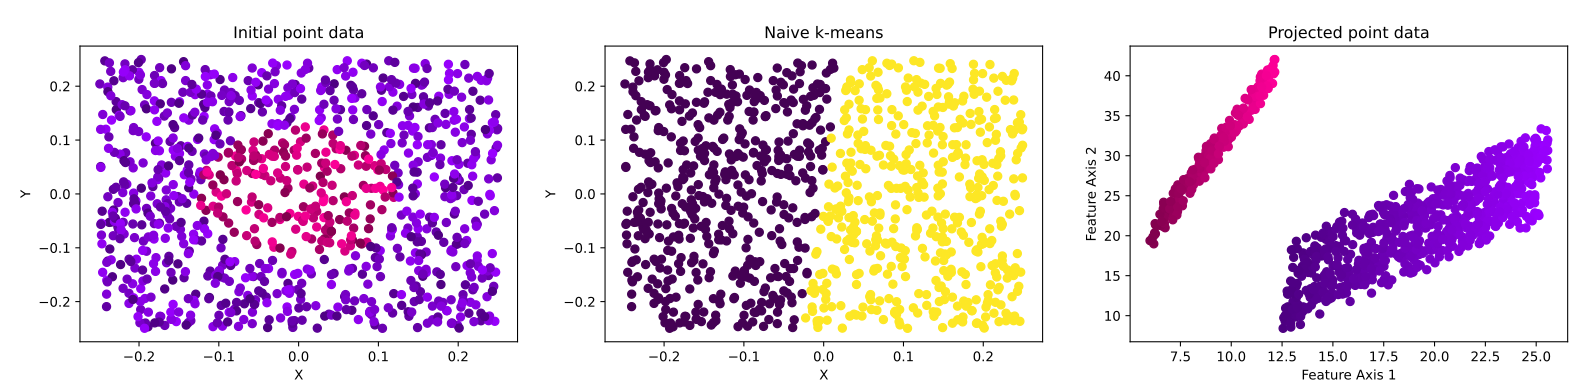
\includegraphics[width=\linewidth]{figures/clustering_color.png}
    \caption{Example of color feature separation in uniform distribution of points in space.}
    \label{fig:cluster_color}
\end{figure}

In order to showcase the spatial feature separation, figure \ref{fig:cluster_space} shows two parallel lines with noise, which are close enough together that k-means would not be able to distinguish between them. However, after projecting to a lower-dimensional space based on feature significance, we get a more distinguished separation. These two cases could be also directly solved by k-means by scaling the data and choosing an appropriate separating axis in the 6-dimensional space, but this algorithm is more robust since the choices for transforming the data are based on the distribution of data in the initial point set. 

\begin{figure}[H]
    \centering
    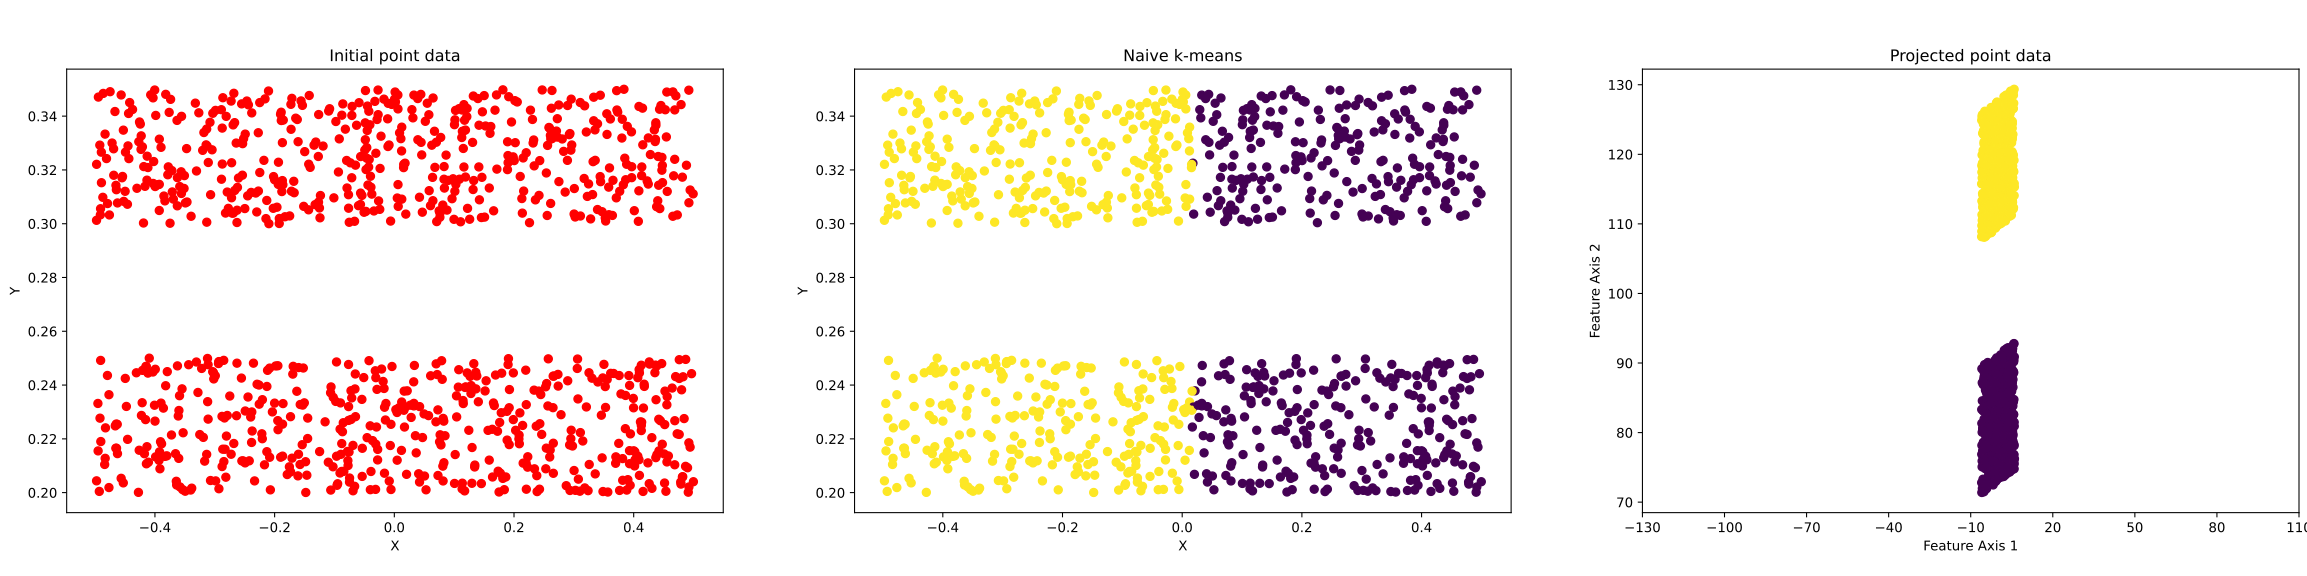
\includegraphics[width=\linewidth]{figures/clustering_space.png}
    \caption{Example of spatial feature separation with uniform color.}
    \label{fig:cluster_space}
\end{figure}

Note that this partitioning approach for the BSP component of the tree does not result in volumetric separation of the primitives, and in some cases, the bounding boxes of the resulting children nodes might have significant overlap. However, this produces significantly better results in terms of image quality. More examples using actual 3DGS scenes will be shown in the Results chapter. 
\newpage
\section{Level of Detail Generation and Selection}
Now that I have presented the methods implemented for space partitioning and Gaussian merging in the previous two chapters, I will discuss how these two concepts are combined to create the acceleration structure. The solution I propose in this project is a view-dependent continuous LoD structure \cite{lod} since the amount of detail is selected dynamically for each frame depending on the camera position relative to scene elements and the desired granularity.

\subsection{Generating the Level of Detail}
The level of detail representation is generated in an incipient step when the scene is loaded into memory. The scene partitioning algorithm begins from the bounding box of the entire scene, generated from the confidence ellipsoids of all Gaussians. The octree component of the hybrid partitioning is built without holding any intermediate information in the nodes, except the connectivity information to the children, as no simplification takes place at this level. For most scenes in my tests, I am using an octree depth of 14, which provides good node uniformity across the scene while leaving enough space for multiple levels of detail in the BSP part. The primitives contained in each node are exclusively passed down to the children based on their location inside the parent node.

\begin{figure}[H]
    \centering
    \makebox[\textwidth][c]{\includesvg[width=0.6\linewidth]{figures/totaltree.svg}}
    \caption{Simplified representation of scene tree showing the different types of nodes and representatives allocation.}
    \label{fig:scenetree}
\end{figure}

When transitioning into the BSP component, the Gaussians are merged from the coarsest nodes to the finer nodes. When a BSP node is processed, all the Gaussians contained in the node are merged using the method presented earlier. The new primitive is added to the list of scene primitives, and its index is stored in the intermediary node. Also at this point, we use the primitives contained in the node to determine the actual bounding box of the node, which is used later for level selection. Then, we determine the two distinct clusters in the data, and the Gaussians are passed down to the two children depending on their respective clusters. The process repeats recursively until we reach the leaf nodes of the tree, which only contain one primitive, and all the intermediary BSP nodes have a reference to their merged Gaussian. From now on, I will refer to merged primitives of interior nodes as \textit{representatives}, as their intended use is to provide a good representation for a set of multiple Gaussians. Compared to other implementations, which build the representations from the finer level to coarse levels by only merging two primitives at a time, I have found that using all Gaussians included in the subtree of a node provides better results when no further training is involved. This means that all representatives are built directly from the original Gaussians, instead of deep intermediary nodes being built by merging two child representatives. Figure \ref{fig:scenetree} shows a simplified representation of the hybrid scene tree.

\subsection{Level Selection}
The second part of the acceleration structure is the level selection. This is done by setting a desired primitive granularity, which dictates which nodes will be passed for render. A larger granularity means that larger intermediary nodes will rasterize their representative, instead of allowing traversal to their children, while a small granularity ensures that the traversal will reach the finer nodes and more primitives will be rendered, resulting in higher quality. The granularity of a node is defined as the approximated area on the screen when the primitive is projected. Because projecting representatives is somewhat costly to be done for all nodes, I am using the bounding box of the node. However, instead of projecting all 8 points of the box and then determining the area, I only compute the projection of its diagonal as if it was viewed perpendicular to the diagonal axis. This metric significantly reduces the overhead when searching for node render candidates and gives a good estimation of the perceived size of a node when projected. Tests using the full box projection showed no improvement in image quality, but the processing time increased significantly.

Given a node with the diagonal of length $d$, the projected size on the screen $d_p$, as defined above, is computed as:
\[
d_p = \frac{d}{D}\frac{W_{screen}}{FOV_y}
\]
where $D$ is the distance from the camera to the node, $W_{screen}$ is the width of the viewport in pixels, and $FOV_y$ is the horizontal field of view of the camera. Figure \ref{fig:granularity} shows a simplified view of this process.

\begin{figure}[H]
    \centering
    \includesvg[width=0.7\linewidth]{figures/granularity.svg}
    \caption{Node granularity computation. The node diagonal is shown in magenta, and its projected length on the image plane is shown in red.}
    \label{fig:granularity}
\end{figure}


The tree traversal starts from the octree leaves, as these mark the roots of the set of BSP subtrees. The tree structure is traversed in a depth-first manner. At each node, we compute the length of its projected diagonal. If the size is larger than the target granularity, the traversal continues to its children, as the node is too large to be rendered directly through its representative. If the projected size is smaller than the granularity, it means that the node satisfies the criterion, its representative is marked for render, and the traversal of that path is terminated (i.e. the node will not add its children to the node processing queue). In case the traversal reaches a leaf, its assigned primitive will be automatically marked for render. This means that setting a target granularity of 0 tells the LoD selection algorithm to render the scene at the highest quality possible. This effectively creates a cut in the tree that marks the nodes that have a granularity smaller than the target granularity, and their immediate parents have a granularity higher than the target granularity.

The intuition behind this approach is that parts of the scene closer to the camera will have a higher projection length, prompting the traversal to advance further into the tree representation and allocate more primitives for rendering that part. Conversely, parts farther away from the camera will have a smaller projection, so they will be simplified more, since the loss of detail in the background is less noticeable, especially when the primitives would only rasterize to a few pixels. However, the higher the detail level, the deeper the traversal has to go inside the scene tree, which means there are higher overheads. These details will be discussed in the Results section.

This section concludes the discussion about generating and using the dynamic level of detail, as I have presented my approach to scene partitioning, Gaussian merging, and lastly how these two combine to create the acceleration structure.
\newpage
\section{Implementation and Performance Considerations}
This section is dedicated to discussing some implementation details, as well as some performance aspects of the implementation considering the target hardware. The implementation of GPU device functions has to take into account overheads introduced by uncoalesced memory accesses, maximizing compute throughput and some other limitations characteristic of the CUDA architecture.

The implementation of the subdivision algorithm and the LoD generation is straightforward, and I did not implement any heavy optimizations because the process only runs once when the scene is loaded, and then the structure is never modified during rendering. This also means that the tree structure can be serialized and written to disk, to facilitate faster loading on subsequent runs. The process could potentially be optimized to run on multiple threads, however, the creation of additional scene primitives implies potentially conflicting writes to the global scene primitive array. There are workarounds to this, like processing subtrees in parallel, and then concatenating their merged primitive vectors, however, this was not the scope of the project, as the overhead can be easily avoided by writing the tree information to disk.

The tree traversal algorithm, however, runs at the beginning of every frame in order to mark the primitives that are eligible for rendering. This means that I have to take special consideration of the performance aspects of the implementation, as overheads that are too large may render this solution ineffective. Because the scene tree is generated in a CPU function call and new nodes are allocated dynamically, we cannot ensure that all the tree data is in a contiguous block of memory after it is generated, as it depends on how the Operating System handles dynamic allocations. After the scene tree is built, I allocate a sufficiently large buffer, traverse the tree, and insert the node information in the buffer, replacing node pointers with buffer indices. This first traversal is also done depth-first, as this is the access pattern when the tree is traversed in the GPU kernel. Now, the tree buffer can be transferred to GPU memory in only one call ensuring memory continuity.

Another significant challenge is the actual tree traversal in the GPU. The CUDA programming model performs well on tasks that perform the same operation on a very large amount of data, and the instructions executed by each thread are mostly the same. Traversing a very deep tree poses problems, as threads in a warp will start to diverge in their execution, which leads to stalls. Also, traversing the entire tree from its root node will pose some issues, as the execution is not parallelizable due to the low amount of concurrent data. To address this issue, I am "splitting" the scene tree at the octree leaf nodes. This means that each subtree starting from an octree leaf node will become an independent structure which will be processed in its entirety by one thread. This results in a large set of shallower trees that are completely independent of one another, so they can be traversed in parallel without issues, and the result of the traversal will be the same as a sequential traversal from the scene root. This optimization takes advantage of the fact that the octree component holds no primitive information and is only used for connectivity information, so it can be ignored in the traversal and we can start directly from the BSP roots.

The changes above ensure that the tree can be traversed in parallel by a large number of threads, but I still have to discuss the actual traversal implementation. Tree and graph-like structures in general are notoriously hard to process in GPU kernels, as there is no effective way to ensure coalesced memory accesses and avoid random memory accesses, which come at a great overhead. Moreover, for this application, the computational load is quite small for every node, as we only compute the length of the projected diagonal, and then decide whether to mark the primitive for render or continue the traversal to the children. This means that memory access overheads will be significant and the compute throughput relatively low. Generally, DFS graph traversals are done with recursive function calls, as the implementation is more elegant and CPUs deal well with relatively large function call stacks. The CUDA framework also allows recursivity through its Dynamic Parallelism functionality. However, this is mostly used to launch a computationally-heavy kernel from an already running kernel. In the traversal case, launching multiple kernels recursively will incur a massive amount of launch overhead for a very short computation. Alternatively, the kernel can be used as a wrapper to a device function implementing recursive calls, but in my experiments, this also performed poorly, and extra care has to be taken not to overflow the call stack.

The most efficient DFS implementation I found for this application is to perform the traversal in a loop, using a stack to keep track of the traversed path. Because the trees are quite shallow in the kernel traversal, allocating a stack of 64 elements is enough to ensure there is no overflow, while also being small enough to fit in the local thread memory for fast access. Using the NVIDIA profiling tools, this method showed the lowest percentage of cache misses and the highest compute throughput (even though the value is lower than ideal in order to take full advantage of the architecture).

The scope of this project is to provide an extension to the existing render pipeline without introducing extensive changes. The existing pipeline remains mostly unmodified, and the traversal is done in a separate kernel call before the pre-processing routine. Marking the primitives eligible for render is done through a boolean mask situated in global GPU memory. The scene tree traversal populates the mask with values, then the mask is passed to the pre-processing routine. Then, the pre-processing will quickly discard the primitives that are not marked for rendering in the mask, and the rest of the pipeline remains unchanged.

\paragraph{}
Another optimization I wanted to explore was performing frustum culling during the traversal. This can easily be performed by intersecting the node bounding box with the frustum planes and eliminating nodes that are out of view by terminating their traversal. The performance obtained from this change is quite mixed and heavily depends on what parts of the scene are in view. First of all, even though frustum intersection is trivial to compute, its computational load inside the kernel is quite significant relative to the other operations that are performed, incurring an increasing cost as the traversal goes deeper into the tree. Secondly, primitives that are out of view are removed early in the pipeline by the pre-processing routine by simply projecting the Gaussian centers to the camera plane and using a heuristic to determine if the projected centers are far enough outside the image plane to be discarded. 

On camera positions that contained the most detailed parts of the scene in view, culling in the traversal did not bring any improvements, and in some cases even incurred a small overhead. The only situation when it is beneficial is when complex parts of the scene are outside the frustum, so many nodes and primitives can be removed early from the traversal by culling large nodes close to the root. Performance metrics and examples of this are discussed in the Results chapter. 
\newpage
\section{Experimental Results}

In this chapter, I will discuss the results obtained using the system developed in this project. First, I will go over intermediate results obtained during development and discuss how these influenced the decisions I took, then present the performance of the final system on multiple scenes. All the experiments that will be presented have been performed on a system running Ubuntu 23.10, with an AMD Ryzen 7 5800H, 16 GB of LPDDR4X RAM, and an NVIDIA RTX 3050 Ti Mobile GPU with 4 GB of VRAM and 2560 CUDA Cores running at 35W. The system configuration is relevant, especially the GPU used, as the performance of the renderer highly depends on the computational capabilities of the graphics card, and the size of some scenes may prevent them from being properly loaded into memory. For reference, most 3DGS publications use the NVIDIA RTX A6000 to test their implementation and generate results. That GPU has an FP32 performance of 38.71 TFLOPS, compared to the hardware I used which only achieves a theoretical maximum of 5.299 TFLOPS, and features 12x more video memory.
\newpage
\section{Conclusions and Future Work}
\subsection{Conclusions}
This thesis presents a solution for accelerating the rendering pipeline for 3D Gaussian Splatting scene representations based on a hierarchical LoD structure which creates intermediary lower-detail representations without additional scene fine-tuning.
\paragraph{}

The main contribution of this work is the space subdivision approach for Gaussian primitives that combines regular subdivision with clustering-based separation, and the solution to merging multiple primitives into one representative Gaussian, especially for estimating the 3D covariance. 
\paragraph{}

Starting from traditional space subdivision algorithms such as octrees and BSP, I evaluated these methods and proposed a hybrid architecture that combines an initial octree subdivision for an even distribution of nodes throughout the scene with a secondary binary partitioning that takes advantage of Gaussian properties to determine their distribution into the children nodes, which leads to better intermediary representation. Also, I justified the choice of the new architecture through experiments showcasing the image quality obtained through each method, eventually showing that this partitioning strategy performs the best for this application.
\paragraph{}

Then, I presented the algorithm used to select the appropriate level of detail for parts of the scene, which is based on a target granularity of the detail. This allows rendering distant parts of the scene in lower detail, as the primitives occupy less space on the screen, thus leaving more resources to be allocated to rendering closer scene components in higher detail. As the granularity of different elements depends on camera position, this creates a dynamic system that chooses the detail levels appropriately for any camera position.
\paragraph{}

Lastly, I presented the results of an extended range of tests covering the achieved image quality metrics, rendering performance, timings of individual routines to evaluate the overheads of this method, memory requirements, and potential benefits of early frustum culling. Moreover, I presented a performance profile of the components of the render loop introduced by me, highlighting potential improvements and steps I took for optimization to achieve the results presented in the previous chapter.
\paragraph{}

To the best of my knowledge, at the time of writing, this is the only proposal for generating LoD representations for 3DGS models without further optimization and fine-tuning. This makes it difficult to evaluate its performance in comparison to other methods. Similar approaches that I presented in the \textit{Related Works} chapter all involve introducing the lower-detail levels in the optimization loop, sometimes even producing image quality results better than the reference implementation using the LoD hierarchy. The performance of my method is also determined by the quality of the initial reconstruction, and reducing the detail can only reduce the quality, as we are only approximating the information that is removed. This is why the method that I presented will have significantly lower quality methods compared to training-based methods and is intended to be used when pre-trained LoDs are not available. 

\subsection{Future Work}
Given the performance results presented in the previous chapter, it is clear that there are more areas of improvement for this solution. Firstly, one of the most important factors in image quality is the primitive separation in nodes, as that ultimately determines the groups merged together. The feature-based clustering proved to be better than basic median splitting, however, the performance could possibly be improved by considering other properties, such as surface normal to determine a primitive grouping that better follows the geometry of the scene. Also, the primitive merging approach is inspired by methods that fine-tune the detail levels, so it is probably not the most optimal for directly displaying the results as representatives. Introducing a few optimization steps based on the perceived effect of specific lower-detail representations could prove beneficial without introducing an overhead that is too big in the generation of the LoD hierarchy.
\paragraph{}

Secondly, the scene tree traversal introduces a significant overhead to the rendering loop, somewhat diminishing the benefits of reducing the number of primitives in the scene. Traversing tree structures on the GPU is not trivial and it usually does not scale well as the amount of data increases. However, there might be better representations of this data in memory to improve contiguity, which seems to be the main issue holding back performance in the current implementation.
\paragraph{}

Lastly, the initial step of subdividing the space and computing the hierarchy of detail levels could be accelerated using parallel computing either on the CPU or on the GPU. As we have seen from the traversal, nodes can be processed in parallel as they do not share any information or dependencies on the same level on the tree. This, however, has not been a priority as the computation is done only once when the scene is loaded and could easily be avoided by storing the new representation to disk for easier loading in subsequent runs.
\paragraph{}

Also, a detail related more to the user experience of moving through the environment rather than the quality of still renders is the transitions between levels. At the moment, the implementation does not feature any mechanism for a smooth visual transition between levels of detail, so there are popping artifacts and parts of the scene transition between levels. This could be alleviated by transitioning between levels for a few frames. However, this would imply rendering more Gaussians than either level consists of during the transition period, which can cause lag spikes during rendering. However, there may be other more appropriate transitioning strategies with better performance, and this is another area of improvement for reducing the amount of visual artifacts.

\newpage
\bibliographystyle{plain} % We choose the "plain" reference style
\bibliography{refs} % Entries are in the refs.bib file

\end{document}
